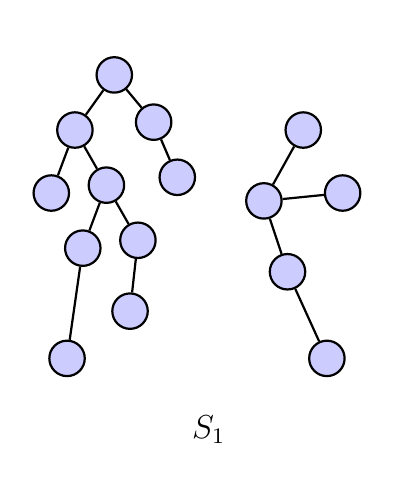
\begin{tikzpicture}[
  baseline=0pt,
  scale=1,
  vnode/.style={circle, draw=black, fill=blue!20, thick, inner sep=0pt, minimum size=4.5mm},
  edge/.style={thick, draw=black}
]
  \useasboundingbox (-2.3,-3.1) rectangle (2.3,2.4);

  % --- ÁRBOL 1 (10 vértices, trazado orgánico) ---
  \node[vnode] (t1_1) at (-1.2, 1.8) {};   % Vértice superior
  \node[vnode] (t1_2) at (-1.7, 1.1) {};
  \node[vnode] (t1_3) at (-0.7, 1.2) {};
  \node[vnode] (t1_4) at (-2.0, 0.3) {};
  \node[vnode] (t1_5) at (-1.3, 0.4) {};
  \node[vnode] (t1_6) at (-0.4, 0.5) {};
  \node[vnode] (t1_7) at (-1.6, -0.4) {};
  \node[vnode] (t1_8) at (-0.9, -0.3) {};
  \node[vnode] (t1_9) at (-1.8, -1.8) {};  % Vértice inferior
  \node[vnode] (t1_10) at (-1.0, -1.2) {};

  \draw[edge] (t1_1) -- (t1_2); \draw[edge] (t1_1) -- (t1_3);
  \draw[edge] (t1_2) -- (t1_4); \draw[edge] (t1_2) -- (t1_5);
  \draw[edge] (t1_3) -- (t1_6);
  \draw[edge] (t1_5) -- (t1_7); \draw[edge] (t1_5) -- (t1_8);
  \draw[edge] (t1_7) -- (t1_9); \draw[edge] (t1_8) -- (t1_10);

  % --- ÁRBOL 2 (5 vértices, trazado orgánico) ---
  \node[vnode] (t2_1) at (1.2, 1.1) {};
  \node[vnode] (t2_2) at (0.7, 0.2) {};
  \node[vnode] (t2_3) at (1.7, 0.3) {};
  \node[vnode] (t2_4) at (1.0, -0.7) {};
  \node[vnode] (t2_5) at (1.5, -1.8) {};   % Vértice inferior

  \draw[edge] (t2_2) -- (t2_1);
  \draw[edge] (t2_2) -- (t2_3);
  \draw[edge] (t2_2) -- (t2_4);
  \draw[edge] (t2_4) -- (t2_5);

  % Etiqueta
  \node[font=\large] at (0,-2.7) {$S_1$};
\end{tikzpicture}
